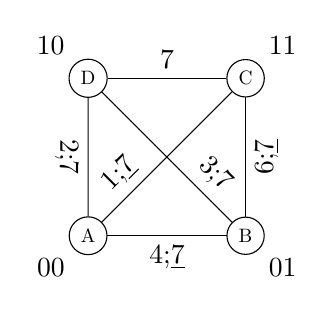
\begin{tikzpicture}[gv/.style={draw=black,circle,scale=0.7},scale=2]
\node[gv] (A) at (0,0) {A}; \draw (A.south west) node[anchor=north east] {$00$};
\node[gv] (B) at (1,0) {B}; \draw (B.south east) node[anchor=north west] {$01$};
\node[gv] (D) at (0,1) {D}; \draw (D.north west) node[anchor=south east] {$10$};
\node[gv] (C) at (1,1) {C}; \draw (C.north east) node[anchor=south west] {$11$};
\draw (A) to node[sloped,below] {4;\underline{7}} (B) to node[sloped,below] {6;\underline{7}} (C) to node[sloped,above] {7} (D);
\draw (B) to node[sloped,above,near start] {3;7} (D) to node[sloped,below] {2;7} (A) to node[sloped,above,near start] {1;\underline{7}} (C);
\end{tikzpicture}